\chapter{Experimental Setup}\label{chap:experimental-setup}
We will now describe how each of the metrics is being captured and what parameters will be used.

\section{Gathering components}\label{sec:experimental-setup:gathering-components}
The SC, CC, LOC, and MA metrics are captured from the source files of components. In order to gather these source files, we do the following: We set up an automatic script that gathers the source files of components on a per-library basis. Since most UI libraries follow the convention of storing each component in a single folder or file in a source folder (generally called \ver{src/} or \ver{components/}), this process is fairly simple. In order to provide a fair comparison, we always select the largest source file for components as the entry point. Some UI libraries use a simple index file that re-exports the actual source file as the entry point. If this file were to be used as the entry point, it would result in an unrealistic depiction of the component source. Since the UI libraries in this study always contain a single big source file, this did not result in any situations where the entry point was ambiguous.

\section{Structural Complexity}
The structural complexity is gathered by capturing the number of imports in a given source file recursively up to a depth of two, as recommended in~\cite{martinez-ortiz2016quality}. To gather these imports, we use the \ver{typescript}\footurl{https://www.npmjs.com/package/typescript} JS package. This package is able to generate an AST or abstract syntax tree of the file. An AST is an in-memory representation of source code. It categorizes the semantic meaning of each expression as a tree, denoting relations between nodes in the tree. By iterating over this tree, we can find the imports. We then follow these imports and apply the same process, filtering out any duplicates.

Similar to~\cite{martinez-ortiz2016quality}, we only apply this process to the JS source code of a component, not the HTML source code. In the case of Svelte components, we separate the file into its JS code and HTML code and apply the process to the JS code only. Code using React is written using either plain JavaScript or JSX. JSX is a superset of JavaScript that supports the describing of HTML elements in JavaScript. Since the \ver{typescript} package has built-in support for JSX, we do not need to separate or modify this code.

\section{Cyclomatic Complexity,Maintainability, Lines of Code}
In order to capture the cyclomatic complexity, maintainability metrics, and lines of code metrics, we input the file into the \ver{ts-complex}\footurl{https://www.npmjs.com/package/ts-complex} JS package. This package is able to calculate the cyclomatic complexity, maintainability metrics, and lines of code of a given source file. Note that the lines of code metric does not capture the raw number of lines but instead filters out any comments, aiming to capture just the lines with actual code.

\section{Machine specifications}\label{sec:experimental-setup:machine-specs}
All experiments were performed on a machine with an AMD Ryzen 5 4600H six-core processor and 16GB of RAM. This machine is running Linux 5.11.15 using the Arch Linux distribution~\footurl{https://archlinux.org/} with mitigations and Meltdown, and Spectre enabled. All experiment data was loaded from an M.2 SSD. Since these experiments are partially timing-specific, the timing-specific experiments were run sequentially and with minimal background tasks. We achieved a state of minimal background tasks by closing off all non-essential tasks in the process manager. This should eliminate the effect of experiments on each other and ensure the CPU can always dedicate a single core to the experiment. Since this machine has six cores, it should easily be able to dedicate one of them to the experiments at all times. Finally, since all experiments were run in one go, the test environments for all tests are identical.

\section{Time-sensitive metrics}\label{sec:experimental-setup:time-sensitive-metrics}
For all time-sensitive metrics (metrics that measure time), we will be taking a few steps to improve their accuracy. We will first of all be artificially slowing down the speed of the processor by a factor of \slowdownFactor{} by using the \code{Emulation.setCPUThrottlingRate} command~\footurl{https://chromedevtools.github.io/devtools-protocol/tot/Emulation/\#method-setCPUThrottlingRate}. We will then divide the measured number by this scale, normalizing the value. Additionally, we will be performing every time-sensitive measure \numMeasures{} times. This allows us to get a good overview of the spread of the measured values, as well as reducing the effect of variations in hardware performance and software influences. Finally, we will be randomizing the order in which tests are run. We do this by creating a queue of all to-be-ran time metrics. Every item in the queue is a single-time metric test for a single bundle, meaning every metric bundle combination will be in the queue \numMeasures{} times. This queue is then shuffled, after which the individual items are executed. While we already made sure to reduce the number of running processes on the benchmark computer, this should ensure that any temporary differences in available processing time should be smoothed out.


\section{Size}\label{sec:experimental-setup:size}
In capturing the size metric, we need to pay attention to several influential factors. The first factor is that the source code of files is split up into multiple files, some of which are not actually used at runtime. Examples of this include files used during testing and definition files. Additionally, it is possible that code does not make it into the bundle because it will not be executed. The process by which code that is not going to be executed is excluded from the resulting bundle is called \emph{tree shaking} and will be discussed later. This means that the size of the source code is not representative of the code that is being used. Additionally, the UI library will have dependencies outside of its source code that also need to be included. To get around this issue, we use a JavaScript bundler. A bundler is a program that bundles all of the source code of a given project into a single file, including dependencies and source files that are being used and excluding unreachable files such as files that contain metadata. We will be using the \ver{esbuild}\footurl{https://esbuild.github.io/} bundler for this process.

Another factor is the way in which the source code is written. A file containing many comments will be larger than a file containing no comments. An increased number of comments in a file does not necessarily indicate increased complexity; if anything, it indicates the opposite. Similarly, longer variable names increase the size as well. To eliminate this factor, we apply \emph{minification} to our bundle. Minification strips out any non-code text from a bundle and reduces the size of the code to the minimum that is needed.

The final factor is the number of components. A UI library with five components will generally be smaller than a UI library with thirty components. Even when we account for this difference by capturing the number of components, the result will still be influenced by the types of components the UI library contains. For example, if two UI libraries are the same except that one of them contains a complex chart component, the library containing the chart will still be bigger on average. This is the case even though any given component in the other library is the same size; the chart library just has more components. To get around this issue, we make use of \emph{tree shaking}. Tree shaking is the process by which unused code is removed from a JS bundle, effectively reducing its contents to just code that is reachable. By marking the same three components as components that should be included in the build for every UI library, we can create bundles containing the same functionality and nothing more.

The tree-shaking process is applicable to the UI libraries against which we are comparing the CC UI library. However, it is not applicable to the CC UI library itself. This is the case because every component is registered as a Web Component simply by loading the library which means that every component is used. This would lead to the CC UI library having a much larger size than other UI libraries. To provide a fair comparison, we will be adding a stripped-down version of the CC UI library to the set of UI libraries against which we are comparing. This stripped-down version only contains the three basic components, and as such, allows for fairer size comparison against other UI libraries.

After these factors are taken care of, the process of capturing the size metric is as easy as getting the size of the resulting bundle.

\section{Load Time}\label{sec:experimental-setup:load-time}
For the load time metric, we will be capturing the parse- and runtime of the JS bundle described in Section~\ref{sec:experimental-setup:size}. We explicitly exclude the network load time of the bundle. In order to collect this metric, we will be using the \ver{puppeteer}\footurl{https://github.com/puppeteer/puppeteer} package. This package allows the running of and programmatic control over a headless instance of the Google Chrome browser~\footurl{https://www.google.com/intl/en_us/chrome/} (a headless browser is a browser without a graphical user interface). We set up an empty webpage containing just the JS bundle whose load time we wish to measure. We then enable the Chrome profiler~\footurl{https://developer.chrome.com/docs/devtools/evaluate-performance/} for the page. The Chrome profiler is a profiler built into the Google Chrome browser that allows for the measuring of various metrics during page execution. For example it is able to measure the run time of JavaScript code and various browser-specific tasks such as painting, compositing and rendering. We now load the page, stop the profiler and collect the results. We then look for the \code{EvaluateScript} event in the resulting trace events. This contains the time taken evaluating the given bundle. An example of such a trace can be seen in Figure~\ref{fig:experimental-setup:load-time}.

\begin{figure}[h]
  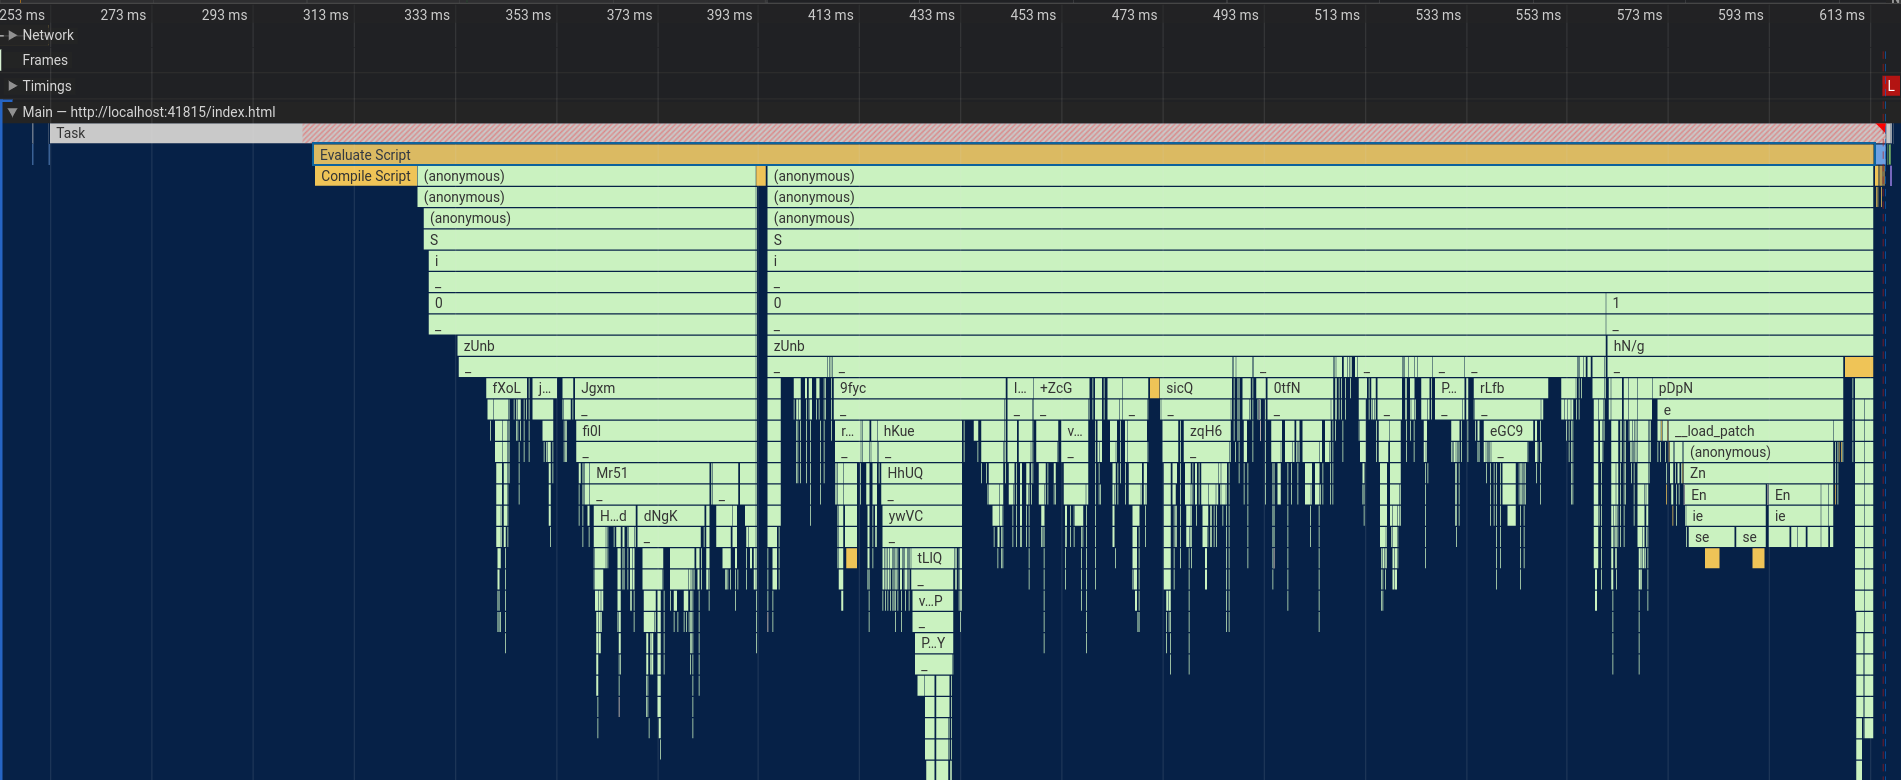
\includegraphics[width=\columnwidth]{figures/experimental-setup/load-time.png}
  \caption{An example of a Chrome profiler trace performed during a bundle load. The orange bar labeled ``Evaluate Script'' indicates the total load time and spans 308.54ms.}
  \label{fig:experimental-setup:load-time}
  \centering
\end{figure}

\section{Render Time}
We capture the render time metric by using the puppeteer package as well. We prepare a JS bundle containing the three basic components and an exposed function that allows them to be rendered on-demand. This function is JS framework-specific since every JS framework has a different method of conditional rendering. The rendering methods for the various frameworks can be seen in Listings~\ref{lst:appendix:react-set-visible},\ref{lst:appendix:angular-set-visible-html},~\ref{lst:appendix:angular-set-visible-js},~\ref{lst:appendix:svelte-set-visible},~\ref{lst:appendix:web-components-set-visible}. We then load the page in a puppeteer browser, enable the profiler, and call the function that renders a given component. We wait for a few seconds, after which we assume the component to be fully rendered. If our assumption turns out to be wrong and the component is not done rendering as we look for the end event, we will be unable to find the end event and metric collecting will fail. We then increase this timeout and try it again. We then iterate through the captured performance trace and look for the time difference between two events. The first event is the calling of the function mentioned above. The second event is the last composite event that has a paint event before it. We repeat this process three times per component (on top of the \numMeasures{} mentioned in Section~\ref{sec:experimental-setup:time-sensitive-metrics}), once with a single instance of the component, once with 10 instances and once with 100 instances. This allows us to measure a more realistic scenario where multiple components are rendered at once, as well as eliminating any performance impacts on just the very first component.

We chose this specific event for the following reason. The chrome browser updates the view through a pipeline process. The complete pipeline can be seen in Figure~\ref{fig:experimental-setup:pipeline}. This process always starts with a JS, CSS, or HTML change. Then it performs a different set of pipeline events depending on what changed.

\begin{figure}[h]
  
\includegraphics[width=\columnwidth]{figures/experimental-setup/render-pipeline.jpg}
  \caption{The render pipeline in chrome.}
  \source{\url{https://developers.google.com/web/fundamentals/performance/rendering}}
  \label{fig:experimental-setup:pipeline}
  \centering
\end{figure}

\begin{itemize}
  \item \emph{Layout:} If a layout property such as the element's dimensions changes, the entire pipeline is run.
  \item \emph{Paint:} If a paint-only property such as a color changes, all but the layout stages run.
  \item \emph{Animation:} If a property that neither layout nor paint changes, only the JavaScript, style, and composite stages run. This pipeline is generally run when an animation is active.
\end{itemize}

In capturing the render time, we want to capture the time until a component reaches its final state. We need to define this final state for all components. While this state is fairly simple to define and is static for most components, it can also be a dynamic final state. For example, a loading spinner or a component that contains a canvas will at some reach its final state but will still be visually changing. The time between the component not being visible and it reaching its final state are spent in the Layout and Paint stages, while the time after it is spent in the Animation stage. Since we want to capture only the time until the final state, we only care about the Layout and Paint stages. The only difference between these two stages and the Animation stage is that the Animation stage ends with a composite event without a paint event before it, and the other two do not. We use this to our advantage by looking for the last composite event that has a paint event before it. We can not just take the lasts paint event since the composite event is still part of the pipeline and is technically part of the render stage. When we take the time between the calling of the function that starts the rendering and this event, we are able to capture the time a component takes to render perfectly. A visual representation of this rendering process can be seen in Figure~\ref{fig:experimental-setup:render-time-start} and Figure~\ref{fig:experimental-setup:render-time-end}.

\begin{figure}[h]
  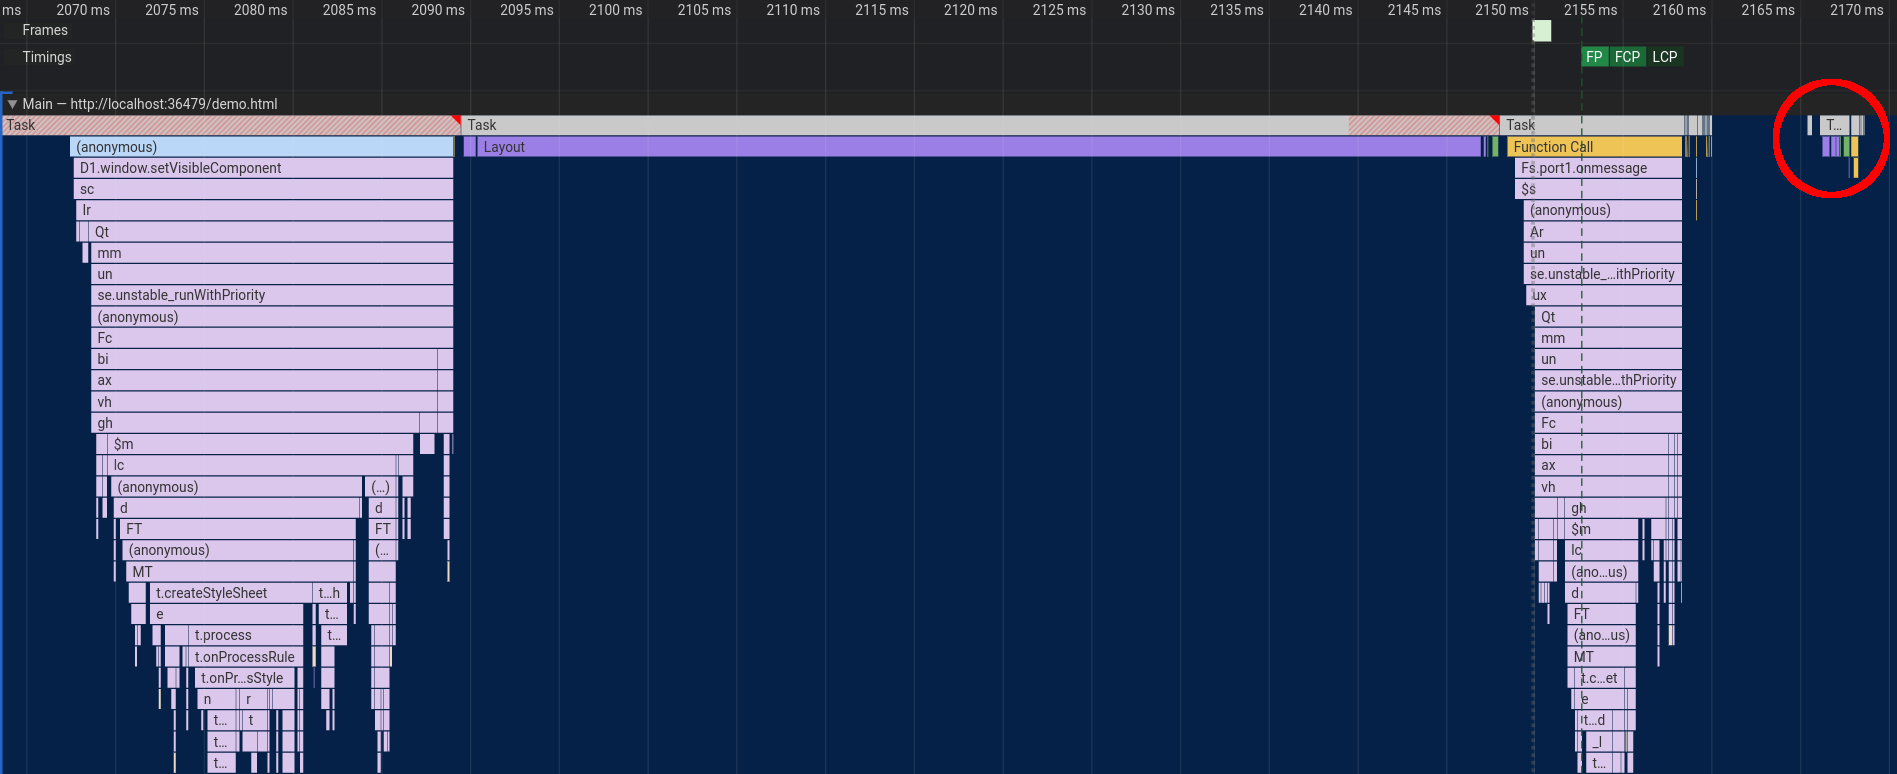
\includegraphics[width=\columnwidth]{figures/experimental-setup/render-time-highlighted.png}
  \caption{An example of a Chrome profiler trace performed during the render of a component. The bar labeled ``window.setVisibleComponent'' indicates our start time. The end time falls within the red circle, a zoomed in version of which can be seen in Figure~\ref{fig:experimental-setup:render-time-end}.}
  \label{fig:experimental-setup:render-time-start}
  \centering
\end{figure}

\begin{figure}[h]
  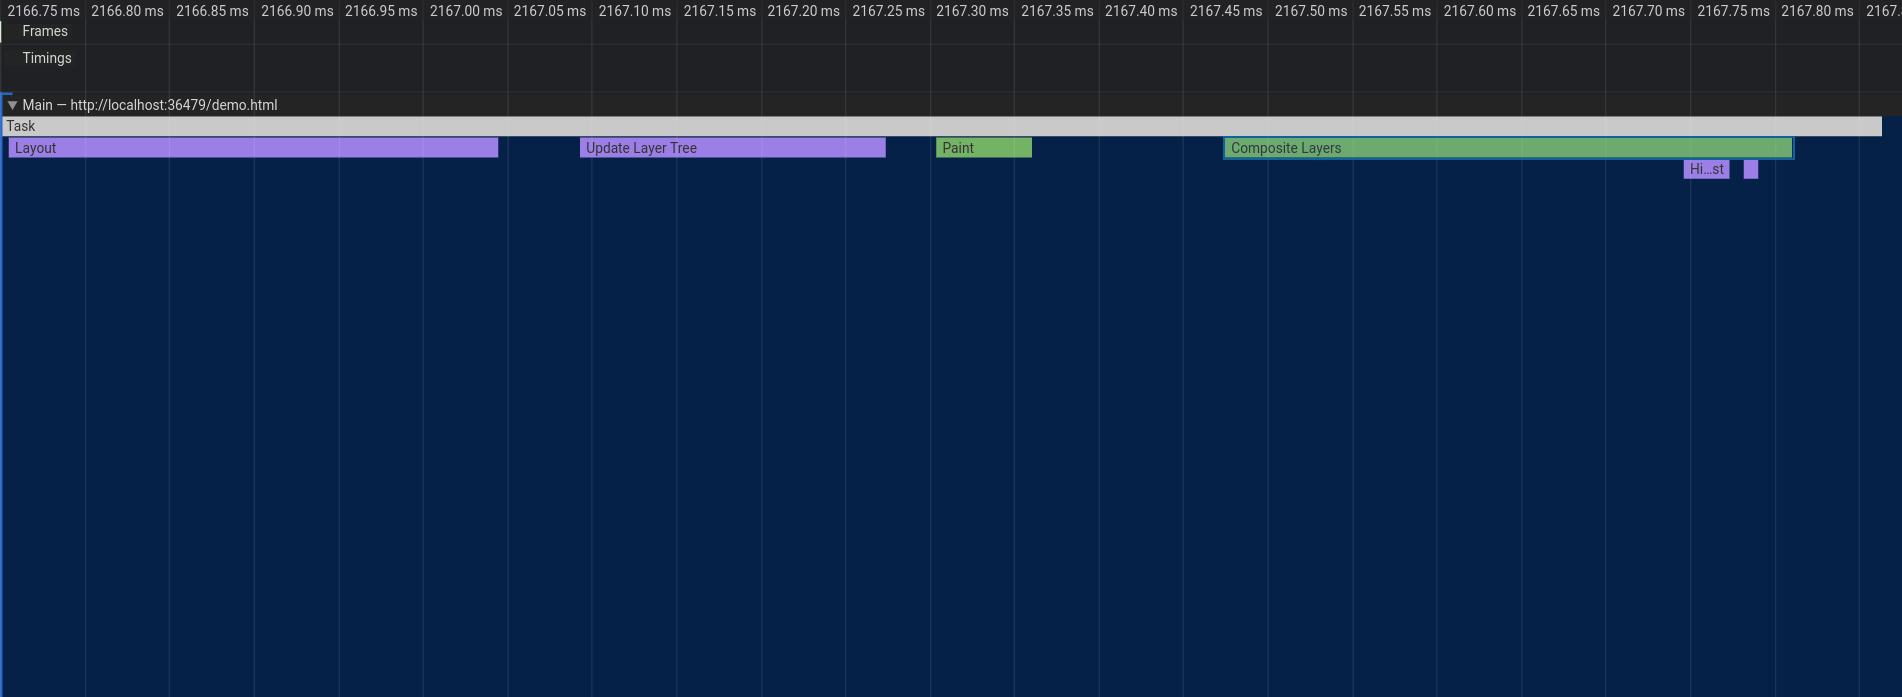
\includegraphics[width=\columnwidth]{figures/experimental-setup/render-time-zoomed.png}
  \caption{An example of a Chrome profiler trace performed during the render of a component. The bar labeled ``composite layers'' signals our end time. Note that this falls just after a bar labeled ``paint'', signaling the paint event before the last composite event.}
  \label{fig:experimental-setup:render-time-end}
  \centering
\end{figure}

\section{First Paint \& First Contentful Paint}
In order to measure the first paint and first contentful paint, we will be constructing a page that has the same content across all versions of the CC UI library. This means we will be constructing one for the original Angular components, the Web Components version, and the various JS framework wrappers. We will be measuring this metric by using the browser's built-in \code{performance} object. This object keeps track of both the FP and FCP metrics, allowing us to extract them.

\section{Number of Components}
The number of components is captured separately for the UI library as a whole and for the bundle described in Section~\ref{sec:experimental-setup:size}. Since the bundles described in Section~\ref{sec:experimental-setup:size} always contain three components, this number will always be three. The only exception is the CC UI library. For the CC UI library and the UI libraries captured as a whole, we will be gathering the number of components by applying the process described in Section~\ref{sec:experimental-setup:gathering-components} to gather components, after which we count the number of them.